\documentclass[11pt,a4paper]{article}

\usepackage[margin=1in]{geometry}
\usepackage{amsmath,amssymb,amsthm}
\usepackage{booktabs}
\usepackage{graphicx}
\usepackage{hyperref}
\usepackage{natbib}
\usepackage{xcolor}
\usepackage{microtype}
\usepackage{setspace}
\usepackage{caption}
\usepackage{subcaption}

\hypersetup{
  colorlinks=true,
  linkcolor=blue!50!black,
  citecolor=blue!50!black,
  urlcolor=blue!60!black
}

\newtheorem{definition}{Definition}
\newtheorem{proposition}{Proposition}
\newtheorem{remark}{Remark}

\title{Fisher Information Loss for Coordination Rules\\
in Decentralized Sensor-Agent Networks}
\author{
  Heath Li\\
  \texttt{Kunyanli230/Jevometry}\\
  \small Working draft toward JAAMAS / arXiv
}
\date{\today}

\begin{document}
\maketitle

\begin{abstract}
Decentralized sensor networks routinely face a last-mile coordination problem:
each mote or edge agent observes only a local reading and a local coordinate,
yet the team must decide \emph{who exchanges what with whom}, and when to
\emph{quarantine} a report under uncertainty. Perception---local categorical
distributions induced by readings and geometry---and coordination---a
deterministic rule that compresses the joint into exchange or quarantine
actions---are often designed separately. While Dec-POMDP active perception
and information-driven sensing carefully treat what to observe, the
coordination layer is frequently heuristic and evaluated only by task reward
or throughput. This paper asks a complementary question: \emph{holding the
agents' local laws fixed, which $\theta$-independent coordination rules
destroy the least Fisher information about the global field or event
parameters?}

We formalize coordination as an AggregationMap $A=f(Z)$ and quantify
information loss by the data-processing gap
$I_Z(\theta)-I_A(\theta)\succeq 0$ between the Fisher information of a
declared product joint and that of its pushforward. Rules are ranked by
$\mathrm{tr}(\Delta)=\mathrm{tr}(I_Z-I_A)$. The intended primary application
is a synthetic unit-disk 2D sensor field (main experiment, forthcoming) with
an Intel Berkeley Lab (IBRL) subnet of motes~$9$--$16$ as a real-data control
(also forthcoming). As a current reproducible analytic instantiation of the
same AggregationMap programme, we use the Jevometry three-agent data-cleaning
council (applicability, repair, risk) and compare seven pure rules---baseline,
stricter, wider, quarantine-to-review, a hybrid quarantine-wider split,
coarse binary, and a near-identity upper bound---on a grid over evidence and
ambiguity. At the design centre, baseline coordination discards roughly half
of $\mathrm{tr}(I_Z)$; softening quarantine into human review recovers a
substantial fraction of that loss, and combining that softening with distinct
auto-normalize/auto-impute labels yields a further improvement that holds on
the full design grid. The ordering
$\mathrm{near\text{-}identity}\le\mathrm{wider}\le\mathrm{baseline}
\le\mathrm{stricter}$
is stable on every grid cell. We discuss design implications for sensor-agent
exchange and quarantine policies, API constraints that force deterministic
maps, and the role of the cleaning numbers as an illustrative proof of
concept pending unit-disk and IBRL results. Accompanying code and reproducible
tables ship with the Jevometry repository.
\end{abstract}

\section{Introduction}

Modern sensing stacks make it cheap for each mote or edge agent to emit a
calibrated-looking categorical distribution over local judgments: observation
quality, whether to report, which neighbour to exchange with, or whether a
reading should be quarantined. In a decentralized sensor network these local
judgments are rarely the end product. A coordinator---often a short piece of
deterministic logic shared by the team---compresses the joint of agent outputs
into exchange decisions (who/what to exchange) or a quarantine safety
valve~\citep{jevometry2026}.

This compression is an information bottleneck. Classical decision theory and
Dec-POMDP planning optimize rewards defined on beliefs or on prediction
quality~\citep{lauri2020prediction,lauri2020decpomdp,oliehoek2016decpomdp}.
Information-theoretic multi-agent sensing maximizes mutual information or
related set functions, often with submodular greedy
guarantees~\citep{krause2008near,nemhauser1978analysis,corah2021scalable,shi2026imas2}.
Those lines of work choose \emph{what to observe} or \emph{who should
observe}. They do not, by themselves, tell a practitioner which of two
already-deployed coordination rules retains more sensitivity to the global
field or event parameters~$\theta$ the network was designed to track.

Fisher information provides a local, differentiable language for that
sensitivity~\citep{fisher1925theory,amari2016information}. For a
discrete model $P_\theta(Z)$ with score Jacobian $J_Z$, the Fisher matrix
$I_Z=J_Z^\top \mathrm{diag}(P_\theta)^{-1} J_Z$ measures how strongly
infinitesimal parameter moves change the outcome distribution. When a fixed
map $f$ produces actions $A=f(Z)$, the data-processing inequality for Fisher
information asserts $I_Z-I_A\succeq 0$ under standard regularity
conditions~\citep{zamir1998fisherdpi,cover2006elements}. The scalar
$\mathrm{tr}(I_Z-I_A)$ is then a comparable loss summary when $I_Z$ is held
fixed.

\paragraph{Target setting and current evidence.}
Our primary narrative is decentralized sensor agents under local observations,
using Fisher~$\Delta I$ as a shared decision function to choose among
coordination rules---including quarantine when uncertain. The intended main
experiment is a synthetic unit-disk field in 2D; a secondary control is the
Intel Berkeley Lab (IBRL) subnet of motes~$9$--$16$. Those sensor experiments
are forthcoming and are \emph{not} reported numerically here. What we
\emph{do} report is a reproducible analytic instantiation of the same
AggregationMap programme: the Jevometry three-agent cleaning council, whose
tables and figures serve as a proof of concept for ranking
\texttt{near}/\texttt{wider}/\texttt{baseline}/\texttt{stricter}/
\texttt{quarantine\_*}/\texttt{near\_identity}-style rules by
$\mathrm{tr}(\Delta)$.

\paragraph{Contributions.}
\begin{enumerate}
  \item We cast multi-agent coordination-rule comparison as ranking
  $\theta$-independent aggregation maps by Fisher information loss under a
  shared declared joint, with sensor-network exchange and quarantine as the
  motivating AggregationMap semantics (Section~\ref{sec:problem}).
  \item We map the programme onto three layers---global field parameters
  $\theta$, local agent categorical laws, and $\theta$-independent
  AggregationMaps---and state the planned unit-disk main experiment and IBRL
  control (Section~\ref{sec:sensor-layers}).
  \item As a current analytic instantiation, we instantiate seven pure rules
  in the Jevometry cleaning council and provide a reproducible harness that
  sweeps a parameter grid, exports CSV/JSON (including parameter-axis loss
  diagonals and fractional losses), and emits publication figures
  (Section~\ref{sec:method}).
  \item Empirically, at the design centre the baseline rule loses about
  $44\%$ of $\mathrm{tr}(I_Z)$; quarantine-to-review cuts loss by roughly a
  quarter relative to baseline; a hybrid quarantine-wider rule improves
  further ($\mathrm{tr}(\Delta)\approx 2.16$) and dominates
  quarantine-to-review on the full grid; a binary gate loses more than
  stricter mid-risk rejection (Section~\ref{sec:experiments}). These numbers
  illustrate the AggregationMap audit; they are not unit-disk or IBRL results.
  \item We discuss how this metric complements reward-centric Dec-POMDP
  evaluation for sensor coordination and what API constraints (deterministic
  maps only) imply for future learned coordinators
  (Section~\ref{sec:discussion}).
\end{enumerate}

This manuscript is intended as a short journal / arXiv draft accompanying
open-source experiments. Cleaning-council numbers are analytic and
illustrative; sensor-field results will replace them as the primary empirical
story once the unit-disk and IBRL harnesses land.

\section{Related work}
\label{sec:related}

\paragraph{Dec-POMDP active perception.}
\citet{lauri2020prediction} reduce multi-agent active perception with
prediction rewards to standard Dec-POMDP solvers via individual prediction
actions, with decentralization-loss bounds. \citet{lauri2020decpomdp}
optimize convex belief-dependent rewards (e.g., negative entropy) with policy
graph improvement in discrete and continuous-state settings. Both lines
typically treat the team as fixed and fold information objectives into
rewards rather than post-hoc comparing deterministic coordinators.

\paragraph{Information-driven multi-agent sensing.}
Submodular sensor selection and multi-robot tracking maximize mutual
information or related coverage objectives with greedy
$(1-1/e)$ guarantees under monotonicity~\citep{krause2008near,corah2021scalable}.
\citet{olkin2024vulcan} and \citet{molloy2023smoother} further connect planning
to information and smoother entropy.

\paragraph{IMAS$^2$ (closest Dec-POMDP relative).}
\citet{shi2026imas2} study \emph{joint} sensing-agent selection and
decentralized active-perception policy synthesis in Dec-POMDPs
(\texttt{arXiv:2510.20009}; AAMAS~2026). An inner layer maximizes mutual
information between latent trajectories (or a secret property) and the team's
partial observations; an outer layer greedily selects agents under
submodularity, with a $(1-1/e)$-style guarantee when successive marginal gains
satisfy their stated ratio condition. Experiments use multi-agent cooperative
perception in a grid world. That programme \emph{optimizes who senses and how}
under Dec-POMDP dynamics. Ours is a related but distinct route: we
\emph{hold} the local agent laws fixed and rank $\theta$-independent
AggregationMaps by Fisher information loss
$\Delta_f=I_Z-I_A$ after action aggregation---including quarantine as a
deterministic safety valve---rather than maximizing mutual information via
submodular agent selection. The two metrics answer complementary questions
(select/synthesize sensors vs.\ audit last-mile coordination).

\paragraph{Information geometry for agents.}
Fisher--Rao geometry supplies local metrics on parametric families of
distributions~\citep{amari2016information}. Jevometry operationalizes node-
and system-level Fisher diagnostics for agent
systems~\citep{jevometry2026}. We use its pushforward
\texttt{information\_loss} primitive and do not modify the underlying
DECLARED\_PRODUCT construction.

\section{Problem formulation}
\label{sec:problem}

\subsection{Declared product joint}

Let $\theta\in\Theta\subset\mathbb{R}^d$ parameterize a multi-agent system.
Each agent $i\in\{1,\ldots,m\}$ emits a categorical distribution
$P_\theta(Z_i)$ over a finite local alphabet $\mathcal{Z}_i$. A
\emph{declared product joint} asserts conditional independence given
$\theta$:
\begin{equation}
  P_\theta(Z=z)=\prod_{i=1}^{m} P_\theta(Z_i=z_i),
  \qquad z=(z_1,\ldots,z_m)\in\mathcal{Z}=\prod_i\mathcal{Z}_i.
\end{equation}
In the cleaning instantiation below, $m=3$, $d=2$, and
$\theta=(\mathrm{evidence},\mathrm{ambiguity})$ with coordinates in
$[0,1]$. In the planned sensor instantiation, $\theta$ instead denotes
global field or event parameters (e.g., source location, intensity, or
event indicators), not raw single-node readings. The product declaration is
an assumption of the model, not an empirical claim about live APIs or radio
traces.

\subsection{Coordination as aggregation}

\begin{definition}[Coordination rule]
A coordination rule is a map $f:\mathcal{Z}\to\mathcal{A}$ into a finite
action alphabet $\mathcal{A}$. We call $f$ \emph{pure} if it is a total
function of the joint outcome alone (no hidden randomness) and
\emph{$\theta$-independent} if $f$ does not depend on $\theta$.
\end{definition}

The induced action law is the pushforward
\begin{equation}
  P_\theta(A=a)=\sum_{z:f(z)=a} P_\theta(Z=z).
\end{equation}
If $J_Z(\theta)$ is the Jacobian of the joint probability vector with respect
to $\theta$, the aggregate Jacobian $J_A$ is obtained by summing rows of
$J_Z$ that share an action label.

\subsection{Fisher information loss}

\begin{definition}[Information loss of a rule]
For a $\theta$-independent rule $f$, define
\begin{align}
  I_Z(\theta) &= J_Z(\theta)^\top \mathrm{diag}\bigl(P_\theta(Z)\bigr)^{-1} J_Z(\theta),\\
  I_A(\theta) &= J_A(\theta)^\top \mathrm{diag}\bigl(P_\theta(A)\bigr)^{-1} J_A(\theta),\\
  \Delta_f(\theta) &= I_Z(\theta)-I_A(\theta).
\end{align}
We report $\mathrm{tr}(I_Z)$, $\mathrm{tr}(I_A)$, and
$\mathrm{tr}(\Delta_f)$ as scalar summaries, and we verify
$\Delta_f\succeq 0$ numerically (PSD check) as a data-processing diagnostic.
\end{definition}

\begin{proposition}[DPI for fixed maps]
Under standard positivity and differentiability conditions, any
$\theta$-independent $f$ satisfies $\Delta_f(\theta)\succeq 0$. Equality
holds when $f$ is injective on the support of $P_\theta$.
\end{proposition}

\begin{remark}
Maps that depend on $\theta$ (soft policies, learned routers conditioned on
parameters) fall outside this guarantee in the Jevometry implementation and
are reported as unsupported. This paper therefore restricts attention to
pure, fully covering, $\theta$-independent rules---the class that matches
typical production if-then coordinators, mote firmware exchange policies, and
the library's AggregationMap contract.
\end{remark}

\paragraph{Comparison principle.}
Fix the agents and the joint construction. Rank rules by
$\mathrm{tr}(\Delta_f)$ (lower is better) or equivalently by
$\mathrm{tr}(I_A)$ (higher is better). Because $I_Z$ is shared, ranking by
loss is identical to ranking by retained information.

\section{Three layers for sensor-agent coordination}
\label{sec:sensor-layers}

The AggregationMap programme admits a three-layer reading that matches
decentralized sensing:

\begin{enumerate}
  \item[(i)] \textbf{Global parameters $\theta$.}
  $\theta$ denotes field- or event-level quantities of interest (source
  location, intensity, spatial covariance hyperparameters, binary event
  indicators), \emph{not} the raw scalar reading at a single mote. Fisher
  loss is measured with respect to this $\theta$.

  \item[(ii)] \textbf{Local agent laws.}
  Each sensor is an agent. Its categorical distribution $P_\theta(Z_i)$ is
  induced by local coordinates and local readings---for example, bins of
  observation quality, a report/hold decision, or a neighbour-choice alphabet
  under a unit-disk communication graph. The declared product joint assembles
  these local laws.

  \item[(iii)] \textbf{AggregationMap as exchange and quarantine.}
  A $\theta$-independent rule $f$ compresses the joint into coordination
  actions: who exchanges with whom, what payload to send, or whether to
  quarantine a report when local uncertainty is high. Candidate families reuse
  the same qualitative knobs studied below---near-neighbour exchange, wider
  neighbourhoods, baseline firmware, stricter thresholds, quarantine variants,
  and a near-identity upper bound---and are ranked by
  $\mathrm{tr}(\Delta_f)=\mathrm{tr}(I_Z-I_A)$.
\end{enumerate}

\paragraph{Planned sensor experiments (no results yet).}
\begin{itemize}
  \item \textbf{Main (forthcoming):} synthetic unit-disk sensors in a 2D
  field. Local alphabets and AggregationMaps will follow layers~(ii)--(iii);
  tables and figures will report $\mathrm{tr}(\Delta)$ rankings once the
  harness is complete. We deliberately omit fabricated unit-disk numbers.
  \item \textbf{Control (forthcoming):} Intel Berkeley Lab (IBRL) subnet,
  motes~$9$--$16$, as a real-deployment sanity check under the same
  AggregationMap interface. Again, no IBRL numbers are claimed in this draft.
\end{itemize}
The cleaning-council study in Sections~\ref{sec:method}--\ref{sec:experiments}
is the present, fully reproducible analytic illustration of layers~(i)--(iii)
with $\theta=(\mathrm{evidence},\mathrm{ambiguity})$ and repair/quarantine
actions standing in for exchange/quarantine semantics.

\section{Method and experimental design}
\label{sec:method}

\subsection{Three-agent cleaning council
(analytic instantiation)}

We reuse the offline Jevometry tutorial
\texttt{examples/three\_agent\_cleaning}~\citep{jevometry2026} as a
proof-of-concept AggregationMap audit---not as a claim about live sensor
fields. Three analytic softmax agents produce distributions for a single
candidate repair of a noisy numeric field:

\begin{center}
\begin{tabular}{lll}
\toprule
Agent & Primitive & Support \\
\midrule
applicability & Noul & $\{\mathrm{false},\mathrm{true}\}$ \\
repair & Choice & $\{\mathrm{normalize},\mathrm{impute},\mathrm{quarantine}\}$ \\
risk & Score & $\{0,1,2\}$ (low/med/high) \\
\bottomrule
\end{tabular}
\end{center}

Local logits are affine in $(\theta-\theta_0)$ around the design centre
$\theta_0=(0.7,0.3)$, and probabilities are obtained by softmax. The joint
is the declared product (ConstructionMode.DECLARED\_PRODUCT). No live API is
queried; no actual database write is performed. Quarantine in this council
plays the same structural role as a sensor quarantine valve: a coarse action
that merges distinguishable joint outcomes and therefore inflates
$\mathrm{tr}(\Delta_f)$ unless softened (e.g., into human review or delayed
exchange).

\subsection{Coordination rules}
\label{sec:rules}

We compare seven rules, all pure and $\theta$-independent:

\begin{description}
  \item[baseline] Reject if inapplicable, quarantine, or high risk; auto-fix
  if normalize and low risk; otherwise human review.
  \item[stricter] As baseline, but medium risk also rejects.
  \item[wider] As baseline rejects; low-risk normalize and impute become distinct
  auto labels (\texttt{auto\_normalize}, \texttt{auto\_impute}).
  \item[quarantine\_review] Quarantine routes to human review instead of reject;
  reject only on inapplicable or high risk.
  \item[quarantine\_wider] Quarantine-to-review combined with wider's dual auto
  labels: the empirically strongest coarse policy in this study.
  \item[coarse\_binary] Reject under baseline reject conditions; otherwise a
  single \texttt{proceed} action (auto-apply and review collapsed).
  \item[near\_identity] One action label per joint outcome tuple (18 labels):
  Fisher retention upper bound under this alphabet.
\end{description}

In sensor language, baseline/stricter/wider correspond to narrower or broader
exchange policies and risk thresholds; quarantine variants are safety valves;
near-identity is an information-retention upper bound rather than a deployable
radio schedule.

\subsection{Harness}

The script \texttt{paper\_experiments.py} builds nodes and joint once, evaluates
$I_Z$, $I_A$, and $\Delta_f$ on an $8\times 8$ grid over
$\mathrm{evidence}\in[0.2,0.9]$ and $\mathrm{ambiguity}\in[0.1,0.8]$, and
additionally records the exact centre $\theta_0$. Outputs:

\begin{itemize}
  \item \texttt{papers/coord-fisher/data/rule\_loss\_grid.\{csv,json\}}
  \item \texttt{papers/coord-fisher/data/center\_summary.json}
  \item \texttt{papers/coord-fisher/data/center\_loss\_anisotropy.csv},
  \texttt{rule\_loss\_anisotropy\_grid.csv}, fractional-loss heatmaps
  \item \texttt{papers/coord-fisher/data/iteration\_summary.json}
  \item Figures~\ref{fig:center}--\ref{fig:masses} under
  \texttt{papers/coord-fisher/figures/}
\end{itemize}

Library code under \texttt{src/jevometry} is unchanged; only example-level
rules and scripts are extended. Unit-disk and IBRL harnesses will reuse the
same AggregationMap and \texttt{information\_loss} interface once available.

\section{Experiments}
\label{sec:experiments}

\subsection{Centre-point ranking}

Table~\ref{tab:center} reports traces at $\theta_0$. All rules return status
\texttt{ok} with PSD loss matrices. The near-identity map loses nothing (up to
numerical noise), confirming the implementation against the equality case of
the DPI. Baseline loses $\mathrm{tr}(\Delta)\approx 3.03$ out of
$\mathrm{tr}(I_Z)\approx 6.84$---about $44\%$. Wider slightly improves on
baseline by preserving distinct auto paths. Stricter mid-risk rejection
increases loss. Softening quarantine into review yields a large practical gain
($\mathrm{tr}(\Delta)\approx 2.27$); stacking that softening with wider's dual
auto labels (\texttt{quarantine\_wider}) improves further to
$\approx 2.16$ and is the best non-identity coarse policy here. Collapsing to
a binary gate is worst among the listed rules ($\approx 3.71$).

\begin{table}[t]
\centering
\caption{Fisher traces at centre $\theta_0=(0.7,0.3)$, sorted by ascending
loss. $|A|$ is the number of actions with positive mass under the pushforward.
Cleaning-council analytic illustration---not unit-disk or IBRL.}
\label{tab:center}
\begin{tabular}{lrrrrl}
\toprule
Rule & $\mathrm{tr}(I_Z)$ & $\mathrm{tr}(I_A)$ & $\mathrm{tr}(\Delta)$ & $|A|$ & Status \\
\midrule
near\_identity & 6.8418 & 6.8418 & 0.0000 & 18 & ok \\
quarantine\_wider & 6.8418 & 4.6816 & 2.1602 & 4 & ok \\
quarantine\_review & 6.8418 & 4.5764 & 2.2654 & 3 & ok \\
wider & 6.8418 & 3.8285 & 3.0133 & 4 & ok \\
baseline & 6.8418 & 3.8080 & 3.0338 & 3 & ok \\
stricter & 6.8418 & 3.4198 & 3.4220 & 3 & ok \\
coarse\_binary & 6.8418 & 3.1296 & 3.7122 & 2 & ok \\
\bottomrule
\end{tabular}
\end{table}

The core ordering highlighted in prior exploratory work remains:
\begin{equation*}
  \mathrm{near\text{-}identity}
  \;\le\;
  \mathrm{wider}
  \;\le\;
  \mathrm{baseline}
  \;\le\;
  \mathrm{stricter}
\end{equation*}
on \emph{every} cell of the $8\times 8$ design grid ($64/64$), not only at the
centre (numerical tolerances $10^{-9}$). Quarantine-to-review inserts
\emph{below} wider on the loss axis; \texttt{quarantine\_wider} inserts still
lower and satisfies
$\mathrm{tr}(\Delta_{\mathrm{quarantine\_wider}})
\le\mathrm{tr}(\Delta_{\mathrm{quarantine\_review}})$
on $65/65$ recorded centre-and-grid evaluations. Coarse binary sits
\emph{above} stricter---an informative deviation from the original four-rule
story.

\begin{figure}[t]
\centering
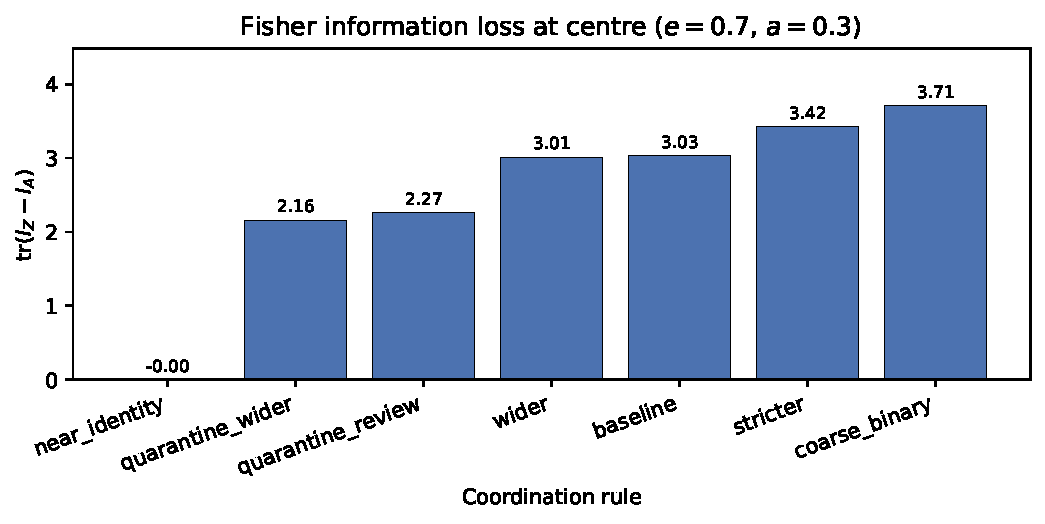
\includegraphics[width=0.85\linewidth]{figures/fig_loss_center.pdf}
\caption{Information loss $\mathrm{tr}(I_Z-I_A)$ by rule at the design centre
(cleaning-council illustration).}
\label{fig:center}
\end{figure}

\subsection{Grid behaviour}

Figure~\ref{fig:heat} shows loss heatmaps for five non-identity rules over the
parameter grid. Absolute loss varies with $\theta$ because both $I_Z(\theta)$
and the mass allocation across $f$-fibres change, but the qualitative ranking
is stable in large regions of the domain: softer, finer action alphabets sit
cooler (lower loss) than stricter or binary gates. Figure~\ref{fig:curves}
slices loss against evidence at ambiguity nearest $0.3$; near-identity stays
at zero, while coarse binary and stricter remain the most lossy.

\begin{figure}[t]
\centering
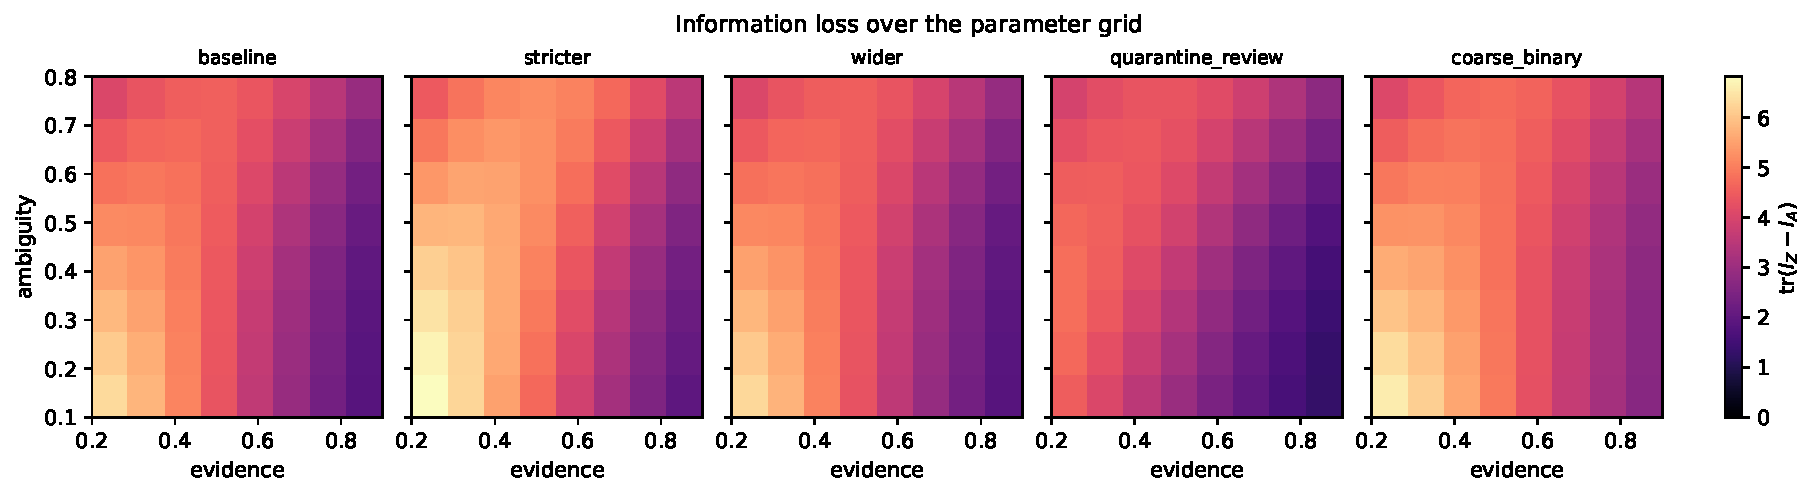
\includegraphics[width=\linewidth]{figures/fig_loss_heatmap.pdf}
\caption{Loss heatmaps over evidence$\times$ambiguity for five coordination rules
(cleaning-council illustration).}
\label{fig:heat}
\end{figure}

\begin{figure}[t]
\centering
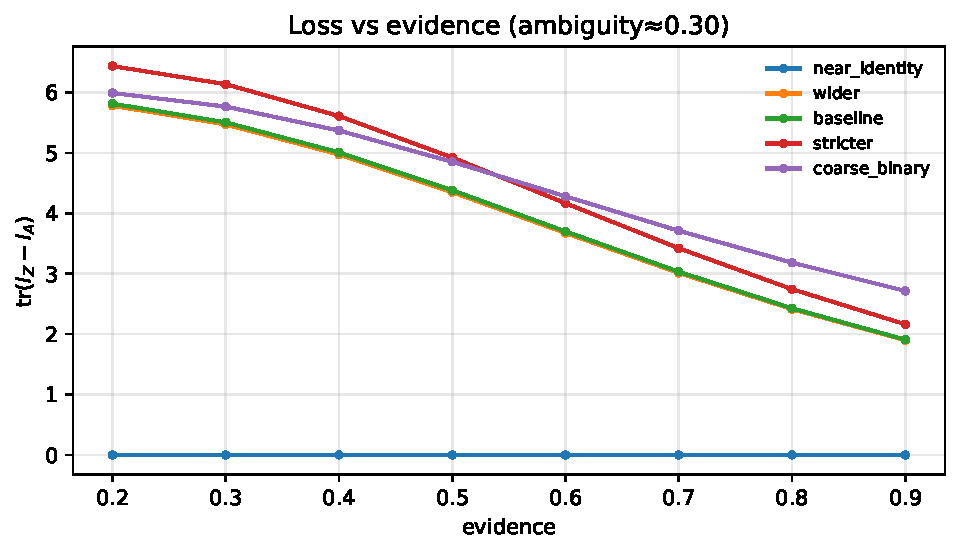
\includegraphics[width=0.85\linewidth]{figures/fig_loss_curves.pdf}
\caption{Loss versus evidence at fixed ambiguity near $0.3$
(cleaning-council illustration).}
\label{fig:curves}
\end{figure}

\subsection{Action masses}

Figure~\ref{fig:masses} shows how probability mass is partitioned at the
centre. Stricter reallocates medium-risk mass into reject. Wider splits
auto-apply into normalize versus impute. Quarantine-to-review shrinks reject
in favour of human review. Coarse binary folds auto-apply and review into
\texttt{proceed}. These mass shifts are the mechanism behind Fisher loss:
merging outcomes with dissimilar score rows collapses distinguishable
parameter directions---the same mechanism AggregationMaps will exhibit when
merging exchange or quarantine fibres in a sensor field.

\begin{figure}[t]
\centering
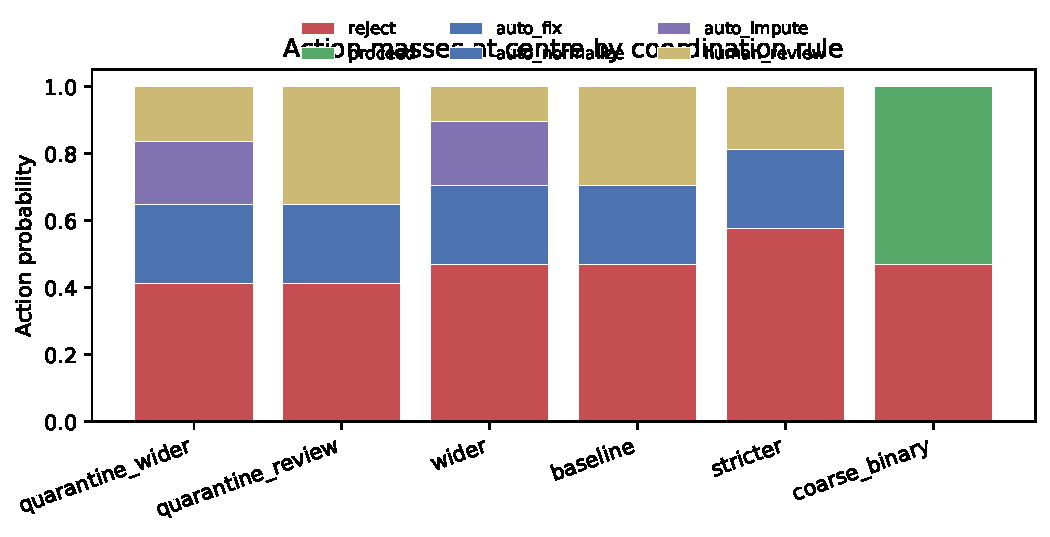
\includegraphics[width=0.85\linewidth]{figures/fig_action_masses.pdf}
\caption{Pushforward action probabilities at the centre for non-identity rules
(cleaning-council illustration).}
\label{fig:masses}
\end{figure}

\subsection{Anisotropy and the quarantine-wider mechanism}
\label{sec:anisotropy}

Trace summaries hide which parameter direction is discarded. At $\theta_0$, the
diagonal entries of $\Delta_f$ in the $(\mathrm{evidence},\mathrm{ambiguity})$
basis show that \texttt{quarantine\_review} cuts ambiguity-axis loss roughly in
half relative to baseline ($\Delta_{aa}\approx 0.95$ vs $\approx 1.69$) while
evidence-axis loss stays comparable. Relative losses
$\mathrm{tr}(\Delta)/\mathrm{tr}(I_Z)$ preserve the same ranking where
$I_Z(\theta)$ varies across the grid.

Pushforward masses explain the hybrid gain: relative to
\texttt{quarantine\_review}, \texttt{quarantine\_wider} replaces a single
\texttt{auto\_apply} atom by distinct \texttt{auto\_normalize} and
\texttt{auto\_impute} atoms and moves additional mass out of
\texttt{human\_review} into \texttt{auto\_impute}; \texttt{reject} mass is
unchanged. Finer auto fibres retain score rows that the coarser review rule
had merged.

\begin{figure}[t]
\centering
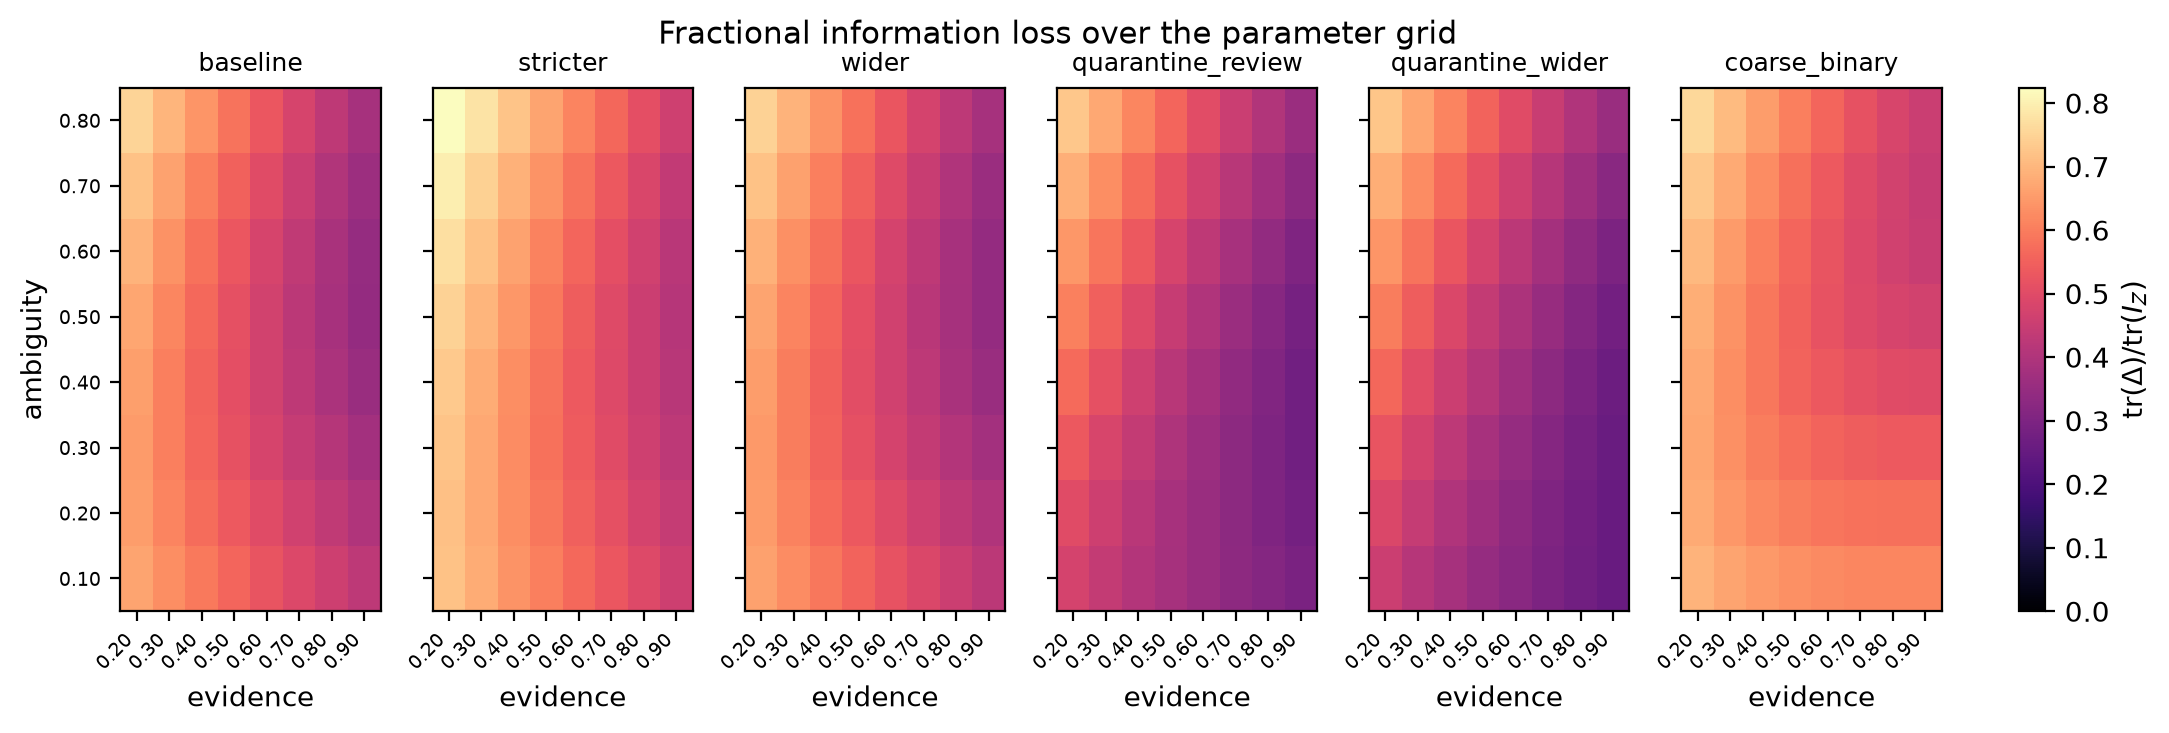
\includegraphics[width=0.9\linewidth]{figures/fig_frac_loss_heatmap.png}
\caption{Fractional loss $\mathrm{tr}(\Delta)/\mathrm{tr}(I_Z)$ over the
evidence$\times$ambiguity grid for non-identity rules
(cleaning-council illustration).}
\label{fig:frac}
\end{figure}

\section{Discussion}
\label{sec:discussion}

\paragraph{Sensor-network reading.}
Under layers~(i)--(iii), $\mathrm{tr}(\Delta_f)$ is a shared offline score for
choosing among exchange and quarantine rules when local agent laws are held
fixed. Softer quarantine (delay or human/operator review instead of hard drop)
and finer exchange alphabets (distinct neighbour or payload labels) are the
direct analogues of the quarantine-wider gains in Table~\ref{tab:center}.
Binary proceed/reject gates remain operationally convenient but
informationally costly. Until unit-disk and IBRL numbers are available, the
cleaning council supplies only qualitative guidance: the ranking machinery and
DPI certificate transfer; the absolute traces need not.

\paragraph{What ``half the Fisher'' means.}
A $44\%$ drop in $\mathrm{tr}(I_Z)$ after baseline coordination does not mean
the system is $44\%$ ``wrong.'' It means that, locally, infinitesimal changes
in the parameters move the final action distribution less than they move the
joint of agent outputs. If a monitoring dashboard only watches action or
exchange rates, it understates how sensitive the underlying agents are. If a
downstream estimator tries to invert actions for $\theta$, it faces a strictly
harder problem than inverting $Z$.

\paragraph{Design takeaway.}
Among implementable three/four-action policies in the cleaning illustration,
routing quarantine to review retained more Fisher than baseline or wider alone;
combining that softening with distinct auto-normalize/auto-impute labels is
strictly better still on this grid. Practitioners can treat
$\mathrm{tr}(\Delta_f)$---and, when needed, its parameter-axis diagonals---as a
cheap offline score when debating rule changes before A/B tests or firmware
flashes.

\paragraph{Relation to Dec-POMDP rewards and IMAS$^2$.}
Prediction rewards and negative-entropy objectives~\citep{lauri2020prediction,lauri2020decpomdp}
optimize perception policies. IMAS$^2$~\citep{shi2026imas2} further couples
agent selection with mutual-information-maximizing sensing policies under
Dec-POMDP dynamics and submodular greedy selection. Our metric does not replace
those programmes; it audits the \emph{last} deterministic compression after
perception (and any selection) is fixed. Selection expands who may observe;
Fisher $\Delta_f$ ranking asks how much of that observation survives a chosen
AggregationMap---including quarantine---at the exchange layer.

\paragraph{API constraints.}
Many agent and mote platforms expose only sampled outcomes plus deterministic
business or firmware rules. Soft, $\theta$-dependent routers would require
either a declared conditional action model or a refusal of the DPI
certificate---exactly the contract encoded by Jevometry's AggregationMap.
Extending the present study to stochastic coordinators is future work and needs
additional regularity.

\section{Limitations}
\label{sec:limitations}

\begin{itemize}
  \item The reported empirical numbers come from hand-specified analytic
  softmax families in the cleaning council, not from fitted live decision
  models, unit-disk fields, or IBRL traces. Absolute traces are illustrative.
  \item Synthetic unit-disk (main) and IBRL motes~$9$--$16$ (control) sensor
  experiments are forthcoming; this draft contains no fabricated results for
  either.
  \item Conditional independence is declared, not tested.
  \item We report parameter-axis diagonals and eigenvalues of $\Delta_f$, but
  full CRLB-style reads would still need an observation likelihood contract
  the cleaning example does not provide.
  \item Action alphabets differ across rules; $\mathrm{tr}(I_A)$ comparisons
  remain meaningful as retained information about $\theta$, but
  interpretations that treat $|A|$ as utility are out of scope.
  \item No human, task-reward, or sensing-accuracy study yet validates that
  lower Fisher loss improves cleaning or field-estimation outcomes.
\end{itemize}

\section{Conclusion}
\label{sec:conclusion}

We proposed ranking multi-agent coordination rules by Fisher information loss
under a shared declared joint, with decentralized sensor-agent exchange and
quarantine as the primary AggregationMap story. Holding local perception
fixed, deterministic coordinators can discard a large fraction of the joint
Fisher trace; small rule edits (quarantine handling, finer action alphabets,
risk or neighbourhood thresholds) move that loss by amounts that are easy to
measure offline. The three-agent cleaning council provides a reproducible
analytic proof of concept---including the stable ordering
$\mathrm{near\text{-}identity}\le\mathrm{wider}\le\mathrm{baseline}
\le\mathrm{stricter}$
and the quarantine-wider gains---while synthetic unit-disk and IBRL
motes~$9$--$16$ experiments remain the intended main and control empirical
pillars once implemented.

Future work includes (i)~completing the unit-disk main experiment and IBRL
control under the same AggregationMap interface, (ii)~replacing analytic
agents with TypeSafe / live decision-model Jacobians where appropriate,
(iii)~stochastic coordinators with explicit conditional action models, and
(iv)~coupling $\mathrm{tr}(\Delta_f)$ with task-level utilities (field
estimation error, cleaning quality) in JAAMAS-style empirical studies.

\section*{Reproducibility}

From the repository root:
\begin{verbatim}
uv sync --locked
uv pip install matplotlib   # paper figures
uv run python examples/three_agent_cleaning/compare_rules.py
uv run python examples/three_agent_cleaning/paper_experiments.py
\end{verbatim}
Artefacts land in \texttt{papers/coord-fisher/data} and
\texttt{figures/}. Cleaning-council tables and figures in this PDF are the
current analytic illustration; unit-disk and IBRL harnesses are forthcoming.
This PDF was built with pdflatex from
\texttt{papers/coord-fisher/main.tex}.

\bibliographystyle{plainnat}
\bibliography{references}

\end{document}
